% =====================================================================
%  PARTS II-VII of the complete magex deck: the simulation engine
%  (included by magex_complete.tex; uses its preamble and colour code)
% =====================================================================

% ---------------------------------------------------------------------
\section{Part II -- The atomistic spin model}
% ---------------------------------------------------------------------

\begin{frame}{From $\J,\Dv,\A$ to a simulation: the full Hamiltonian \src{spinmodel.py, terms.py}}
\begin{eqbox}[Atomistic Hamiltonian (meV), every ordered pair counted once]{cJ}
\vspace{-2pt}
\[
\cE{E}[\{\e\}] = \sum_i \e_i\!\cdot\!\A_i\!\cdot\!\e_i
 - \sum_{i\neq j} \e_i\!\cdot\!\J_{ij}\!\cdot\!\e_j
 - \sum_{i\neq j}\cJ{B}_{ij}(\e_i\!\cdot\!\e_j)^2
 - \cJ{K_4}\!\!\sum_{\square}\!\big[(\e_i\!\cdot\!\e_j)(\e_k\!\cdot\!\e_l)+(\e_j\!\cdot\!\e_k)(\e_l\!\cdot\!\e_i)-(\e_i\!\cdot\!\e_k)(\e_j\!\cdot\!\e_l)\big]
\]
\[
 + \sum_i\Big[\cJ{K_c}\!\sum_{a<b}\alpha_a^2\alpha_b^2 - \cJ{K_2}(\e_i\!\cdot\!\cR{\bm u})^4 - \cJ{K_3}(\e_i\!\cdot\!\cR{\bm u})^6\Big]
 - \mu_B\sum_i\mu_i\,\e_i\!\cdot\!\cH{\bm B}
 - \frac{\mu_B}{2}\sum_i \mu_i\,\e_i\!\cdot\!\cH{\bm B}^{\rm dip}_i
\]
\end{eqbox}
\begin{columns}[T]
\column{0.5\textwidth}
\small
\begin{itemize}
\item $\J_{ij} = J_{ij}\mathbb 1 + \J^{S}_{ij} + \J^{A}_{ij}$, with $\e_i\!\cdot\!\J^A_{ij}\!\cdot\!\e_j = \Dv_{ij}\!\cdot\!(\e_i\times\e_j)$
\item $\alpha_a = \e_i\!\cdot\!\cR{\bm c}_a$ (cubic axes); $\cJ{K_c}>0$: easy $\langle100\rangle$
\item $J>0$ ferromagnetic; $-J'\sum_{\langle ij\rangle}\Leftrightarrow J=J'/2$
\end{itemize}
\column{0.5\textwidth}
\begin{plainbox}{cH}
\small Effective field (tesla), used by every solver:
\[\cH{\bm B}_i = -\frac{1}{\mu_B\mu_i}\frac{\partial\cE{E}}{\partial\e_i}\]
For the bilinear part $\partial\cE E/\partial\e_i = -2\sum_j\J_{ij}\e_j + 2\A_i\e_i$ (using $\J_{ji}=\J_{ij}^T$).
\end{plainbox}
\end{columns}
\end{frame}

\begin{frame}{Building nanostructures \src{structure.py}}
\begin{columns}[T]
\column{0.52\textwidth}
\small
\textbf{Carving.} A boolean mask on the supercell removes sites and all couplings that touch them:
\[
\J \;\to\; P^T\J P,\qquad P = \text{selection of kept rows/cols (3 per site)}
\]
shapes: sphere, cylinder, cube, ellipsoid, truncated octahedron; vacancies; Voronoi roughness.

\medskip
\textbf{Materials.} Label $m_i$ per site; interface exchange
\[
\J_{ij} \;\to\; \cJ{f}_{m_i m_j}\,\J_{ij}\qquad(\cJ f<0:\ \text{AF interface, exchange bias})
\]
plus per-material moment, $\A$, $K_c$, $K_{2,3}$, damping $\alpha$, temperature.
\column{0.46\textwidth}
\begin{eqbox}[Néel surface anisotropy (VAMPIRE convention)]{cJ}
\small
\[
\cE{E}_i^{\rm s} = \frac{\cJ{k_s}}{2}\sum_{j\in nn(i)}(\e_i\!\cdot\!\hat{\bm r}_{ij})^2
\]
only on sites with fewer neighbours than the bulk. It is a quadratic form, folded into the single-ion tensor:
\[
\A_i \;\leftarrow\;\A_i + \frac{\cJ{k_s}}{2}\sum_{j}\hat{\bm r}_{ij}\hat{\bm r}_{ij}^{T}
\]
so LLG, MC, GNEB and the Hessians see it with no extra code.
\end{eqbox}
\small Pinned spins: zero torque, zero noise, excluded from MC. Temperature profiles: a site temperature $T_i$ in the noise and in $\beta_i$.
\end{columns}
\end{frame}

\begin{frame}{Dipole--dipole interaction by FFT \src{terms.py: Dipolar}}
\begin{columns}[T]
\column{0.55\textwidth}
\small
\[
\cH{\bm B}^{\rm dip}_i = \frac{\mu_0\mu_B}{4\pi}\sum_{j\neq i}\mu_j\,\frac{3(\e_j\!\cdot\!\hat{\bm r})\hat{\bm r}-\e_j}{r^3},\quad \bm r = \bm r_j-\bm r_i
\]
For sublattices $s,t$ on the supercell grid this is a convolution
\[
\cH{\bm B}_s(\bm R) = \sum_{\bm o}\cK{W}_{st}(\bm o)\,\mu_t\e_t(\bm R-\bm o),\qquad
\bm r = -\bm o\cdot\mathbf a + \bm b_t - \bm b_s
\]
evaluated with real FFTs (zero padding on open axes).
\begin{plainbox}{cJ}
\footnotesize The sign of $\bm o$ in $\bm r$ matters only when $\bm b_t\neq\bm b_s$: the direct-sum test
found and fixed this for multi-sublattice systems (error $<10^{-15}$ now).
\end{plainbox}
\column{0.43\textwidth}
\small\textbf{Periodic axes.} All image vectors inside a sphere $|\bm r|\le R_c$ are summed, so each is counted once.
For a film the remaining sheets are added analytically:
\[
\int_{R_c}^\infty\!\!2\pi r\,dr\,\frac{\langle 3\cos^2\varphi-1\rangle}{r^3}=
\begin{cases}+\pi/R_c & \e\parallel\text{plane}\\ -2\pi/R_c & \e\perp\text{plane}\end{cases}
\]
\[
\cK{W}^{\rm tail} = \frac{\mu_0\mu_B}{4\pi}\frac{\pi}{A_{\rm cell}R_c}\big(\mathbb 1 - 3\hat{\bm n}\hat{\bm n}^T\big)
\]
relative error $10^{-4}$ at 2 shells, $4\times10^{-6}$ at 8 (vs $10^{-2}$ without the tail).
\end{columns}
\end{frame}

\begin{frame}{Dipolar sums: convergence and shape anisotropy}
\centering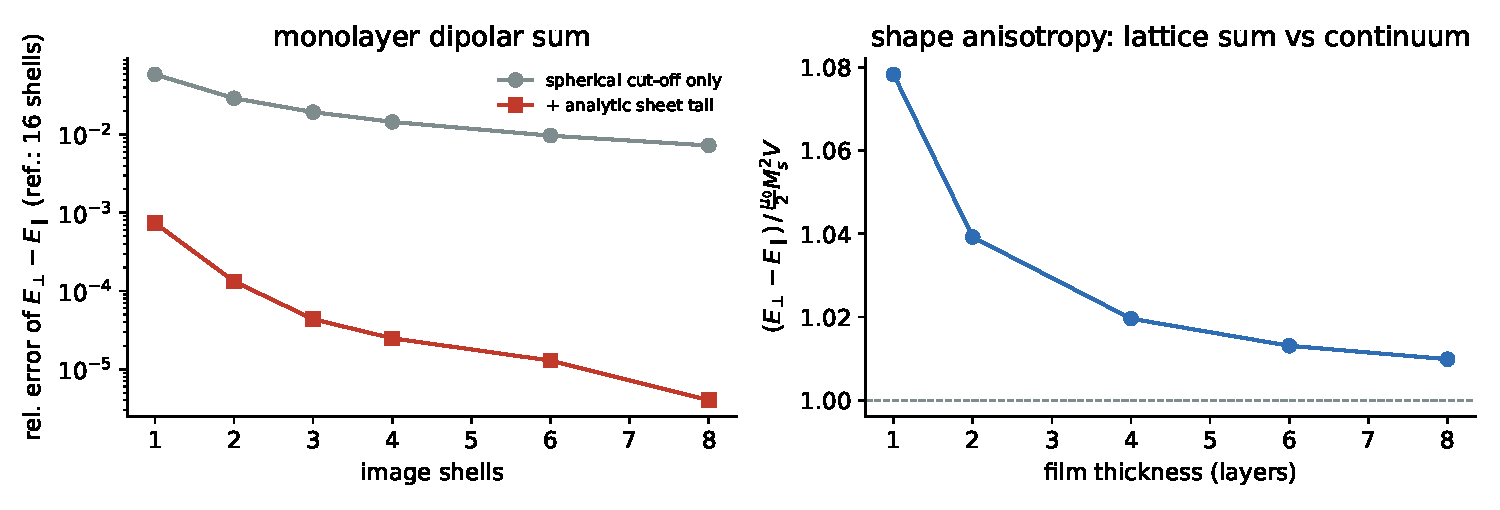
\includegraphics[width=0.9\textwidth]{figs/eng_dipolar.pdf}
\takeaway{the lattice sum reproduces the continuum shape anisotropy $\tfrac{\mu_0}{2}M_s^2V$ for thick films and the correct monolayer value; the sheet tail makes images converge fast.}
\end{frame}

\begin{frame}{Initial textures \src{structure.py: init\_texture}}
\begin{columns}[T]
\column{0.52\textwidth}
\small
\textbf{Skyrmion} (radius $R$, wall $w$, polarity $p$, vorticity $v$, helicity $\eta$):
\[
\cR\theta(r) = 2\arctan\frac{\sinh(R/w)}{\sinh(r/w)},\quad \cR\phi = v\,\psi + \eta
\]
\[
\e = (\sin\cR\theta\cos\cR\phi,\ \sin\cR\theta\sin\cR\phi,\ p\cos\cR\theta)
\]
$\eta=$ \texttt{"auto"} picks among $0,\pi,\pm\pi/2$ the one with the lowest $\cE E$.
Topological charge $Q = \frac{1}{4\pi}\int\e\cdot(\partial_x\e\times\partial_y\e)$: $|Q|=1$, $Q\to-Q$ for $v=-1$.

\medskip
\textbf{Spiral} $\e = \cos(\bm q\cdot\bm r)\hat{\bm n} + \sin(\bm q\cdot\bm r)\hat{\bm q}$ (cycloid) or helix.
\column{0.46\textwidth}
\small
\textbf{Hopfion}: stereographic projection and Hopf map, $\bm r/R\mapsto(z_1,z_2)\in\mathbb C^2$,
\[
z_1 = \frac{2(x+iy)/R}{1+r^2/R^2},\ z_2=\frac{2z/R + i(r^2/R^2-1)}{1+r^2/R^2}
\]
\[
\e = \big(2\,\mathrm{Re}\,z_1\bar z_2,\ 2\,\mathrm{Im}\,z_1\bar z_2,\ |z_2|^2-|z_1|^2\big)
\]
\textbf{Domain wall}: $\cR\theta(x) = 2\arctan e^{(x-x_0)/w}$, Néel or Bloch.
\end{columns}
\end{frame}

% ---------------------------------------------------------------------
\section{Part III -- Spin dynamics}
% ---------------------------------------------------------------------

\begin{frame}{Stochastic Landau--Lifshitz--Gilbert equation \src{llg.py}}
\begin{eqbox}[sLLG, Landau--Lifshitz form]{cR}
\[
\frac{d\e_i}{dt} = -\frac{\gamma}{1+\alpha_i^2}\Big[\e_i\times(\cH{\bm B}_i+\cE{\bm b}_i) + \alpha_i\,\e_i\times\big(\e_i\times(\cH{\bm B}_i+\cE{\bm b}_i)\big)\Big]
\]
\end{eqbox}
\begin{columns}[T]
\column{0.5\textwidth}
\small
Brown's thermal field from the fluctuation--dissipation theorem:
\[
\langle \cE{b}_{ia}(t)\,\cE{b}_{jb}(t')\rangle = \frac{2\alpha_i k_BT_i}{\gamma\mu_i\mu_B}\,\delta_{ij}\delta_{ab}\delta(t-t')
\]
discretised as $\cE{\bm b}_i = \sigma_i\bm\xi$, $\sigma_i^2 = 2\alpha_ik_BT_i/(\gamma\mu_i\mu_B\Delta t)$, $\bm\xi\sim\mathcal N(0,1)^3$.
The noise is multiplicative $\Rightarrow$ Stratonovich calculus; the stationary distribution is $e^{-\cE E/k_BT}$ on $(S^2)^N$.
\column{0.48\textwidth}
\begin{plainbox}{cK}
\small\textbf{Units.} t in ps, B in T, E in meV, $\gamma = 0.17609$ rad ps$^{-1}$T$^{-1}$, $\mu_B = 0.057884$ meV/T.\\[3pt]
Per-site $\alpha_i$ (materials), site temperatures $T_i$ (gradients, laser spots), pinned sites ($\cH{\bm B}_i=\cE{\bm b}_i=0$).
\end{plainbox}
\end{columns}
\end{frame}

\begin{frame}{Integrators on the sphere}
\small
Write the right-hand side as a tangent vector $\bm f_i(\e)$ and the equivalent rotation vector $\cR{\bm\omega}_i = \e_i\times\bm f_i$ (then $\cR{\bm\omega}\times\e = \bm f$).
\begin{columns}[T]
\column{0.5\textwidth}
\begin{eqbox}[Heun (default), Stratonovich-consistent]{cR}
\footnotesize
$\tilde\e = \mathcal N[\e + \Delta t\,\bm f(\e,\cE{\bm b})]$,\\
$\e' = \mathcal N\big[\e + \tfrac{\Delta t}{2}(\bm f(\e,\cE{\bm b})+\bm f(\tilde\e,\cE{\bm b}))\big]$
\end{eqbox}
\begin{eqbox}[Depondt--Mertens: Heun on rotations]{cR}
\footnotesize
$\tilde\e = \mathcal R(\Delta t\,\cR{\bm\omega}(\e))\,\e,\quad \e' = \mathcal R\big(\tfrac{\Delta t}{2}[\cR{\bm\omega}(\e)+\cR{\bm\omega}(\tilde\e)]\big)\,\e$\\
Rodrigues: $\mathcal R(\bm w)\e = \e\cos w + (\hat{\bm w}\times\e)\sin w + \hat{\bm w}(\hat{\bm w}\cdot\e)(1-\cos w)$
\end{eqbox}
\column{0.48\textwidth}
\begin{eqbox}[Semi-implicit midpoint (SIB, Mentink et al.)]{cR}
\footnotesize
$\e' - \e = \Delta t\,\cR{\bm\omega}(\bar\e)\times\frac{\e+\e'}{2}$ solved exactly by the Cayley transform
\[
\e' = \e + \frac{\bm a\times\e + \tfrac12\bm a\times(\bm a\times\e)}{1+|\bm a|^2/4},\quad \bm a = \Delta t\,\cR{\bm\omega}
\]
norm-preserving, time-reversible.
\end{eqbox}
RK4 and Euler are available for deterministic runs.
\end{columns}
\end{frame}

\begin{frame}{Integrator accuracy and the thermal-field generator}
\centering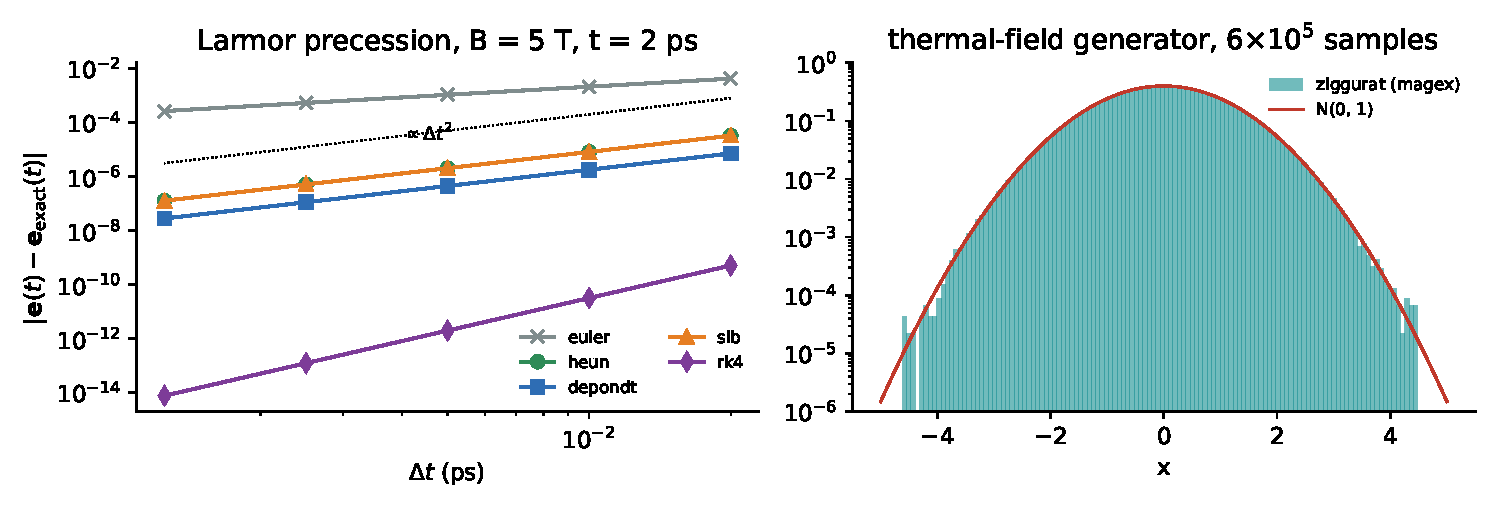
\includegraphics[width=0.92\textwidth]{figs/eng_integrators.pdf}
\takeaway{Heun, Depondt and SIB are second order; the ziggurat generator reproduces the Gaussian down to $10^{-6}$ probability density (tails matter for rare thermal events).}
\end{frame}

\begin{frame}{Quantum thermostat \src{quantum.py}}
\begin{columns}[T]
\column{0.55\textwidth}
\small
Classical noise populates every magnon with $k_BT$. Replace the white spectrum by Bose statistics (no zero-point term):
\[
S(\omega) = 2D\,\frac{x}{e^x-1},\qquad x=\frac{\hbar\omega}{k_BT}
\]
represented as a positive mixture of Ornstein--Uhlenbeck processes and damped oscillators,
\[
\frac{x}{e^x-1}\simeq\sum_k w_k\frac{g_k^2}{g_k^2+x^2} + \sum_l v_l\frac{\Omega_l^4}{(\Omega_l^2-x^2)^2+\Gamma_l^2x^2}
\]
(NNLS fit, error $\sim2\times10^{-3}$ on $[0,30]$); every mode integrated exactly over $\Delta t$.
\column{0.43\textwidth}
\begin{eqbox}[RPA (Tyablikov) ordering temperature]{cE}
\small
\[
k_BT_{\rm RPA}=\frac23\Big[\frac{1}{nN_q}\sum_{\bm q}\mathrm{Tr}\big(\cK D-\tilde{\J}(\bm q)\big)^{-1}\Big]^{-1}
\]
$\tilde J_{ij} = s_is_jJ_{ij}$, $\cK D_{ij}=\delta_{ij}\sum_l\tilde J_{il}(0)$ + anisotropy gap; quantum spins: $T\,(S+1)/S$.
\end{eqbox}
\end{columns}
\end{frame}

\begin{frame}{Spin-transfer and spin--orbit torques on a lattice \src{llg.py, structure.py}}
\begin{columns}[T]
\column{0.53\textwidth}
\small
\textbf{Zhang--Li} (Gilbert form): $\bm T = -(\bm u\!\cdot\!\nabla)\e + \beta\,\e\times(\bm u\!\cdot\!\nabla)\e$.
Solving $\dot\e = -\gamma\e\times\cH{\bm B} + \alpha\e\times\dot\e + \bm T$ for $\dot\e$:
\[
\dot\e = \frac{1}{1+\alpha^2}\big[-\gamma\e\times\cH{\bm B} - \gamma\alpha\,\e\times(\e\times\cH{\bm B}) + \bm T + \alpha\,\e\times\bm T\big]
\]
\textbf{Gradients on any lattice}: least squares over the exchange neighbours,
\[
(\cK{D}_a\e)_i = \sum_j c^a_{ij}(\e_j-\e_i),\ \ c^a_{ij} = w_{ij}\big[\cK M_i^{+}\bm d_{ij}\big]_a,\ \cK M_i = \sum_j w_{ij}\bm d_{ij}\bm d_{ij}^T
\]
(sparse, exact for linear fields, works for carved shapes).
\column{0.45\textwidth}
\small
\textbf{SOT / Slonczewski} as fields: $\cH{\bm B} \mathrel{+}= B_{\rm DL}\,\e\times\bm p + B_{\rm FL}\,\bm p$.\\[4pt]
\textbf{1D wall model}, hard-axis field $B_\perp$, below Walker breakdown:
\[
v = \frac{\beta}{\alpha}\,u,\qquad u_W = \frac{\alpha\gamma B_\perp\Delta}{2|\alpha-\beta|}
\]
\textbf{Two-temperature model}: $C_e\dot T_e = -G(T_e-T_l)+P(t)$, $C_l\dot T_l = G(T_e-T_l)$; the spins see $T_e(t)$.
\end{columns}
\end{frame}

\begin{frame}{Torque dynamics and resonance}
\centering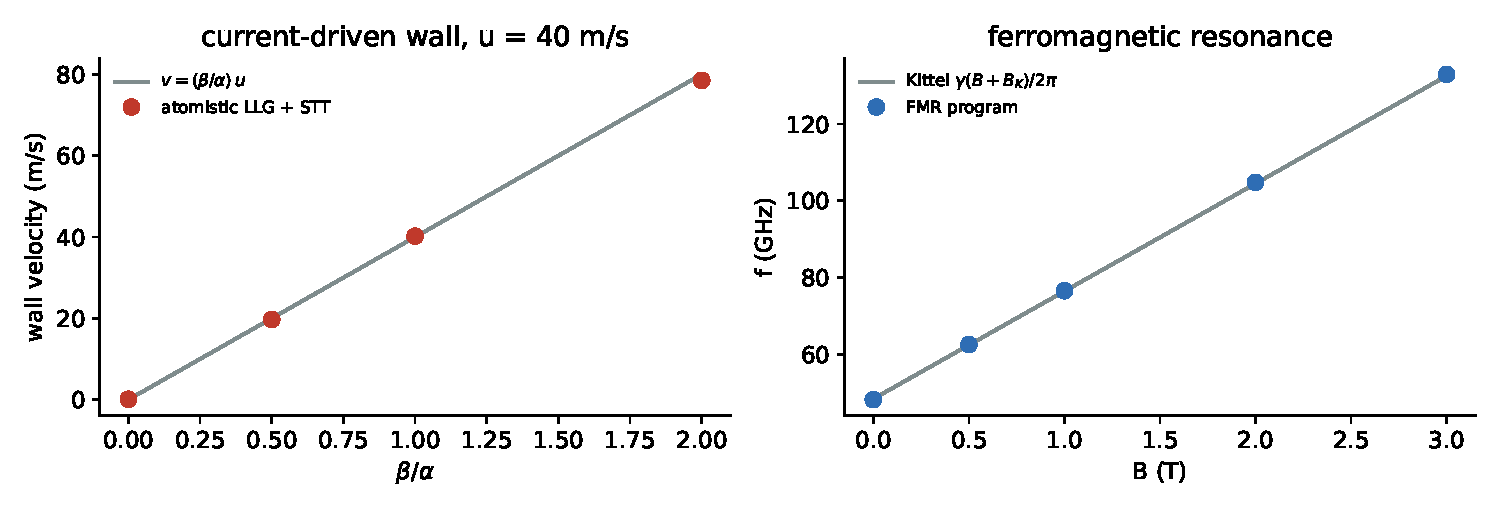
\includegraphics[width=0.92\textwidth]{figs/eng_torques.pdf}
\takeaway{the atomistic Zhang--Li torque gives $v=(\beta/\alpha)u$ to 2\%, and the FMR program the Kittel frequency $\gamma(B+B_K)/2\pi$.}
\end{frame}

\begin{frame}{Longitudinal spin dynamics \src{lsd.py}}
\begin{columns}[T]
\column{0.55\textwidth}
\small
Moments $\bm M_i = s_i\e_i$ with a Landau term (Ma \& Dudarev):
\[
\cE E = \cE E_{\rm spin}[\bm M] + \sum_i\big(a_i s_i^2 + b_i s_i^4\big),\quad a_i = \bm h_i\!\cdot\!\e_i^{\rm ref} - 2b_i
\]
($a_i$ chosen so that the $T=0$ reference has $s_i=1$). Langevin equation:
\[
\dot{\bm M}_i = -\gamma\bm M_i\times\cH{\bm B}_i + \lambda\cH{\bm H}_i + \cE{\bm\xi}_i,\quad \cH{\bm H}_i = -\frac{\partial\cE E}{\partial\bm M_i}
\]
$\langle\cE\xi\cE\xi\rangle = 2\lambda k_BT$. Additive noise: Itô = Stratonovich.
\column{0.43\textwidth}
\begin{proofbox}[Why the ensemble is $e^{-E/k_BT}\,d^3M$]
\footnotesize
Fokker--Planck: $\partial_tP = -\nabla\!\cdot\!(\bm v P) + \lambda\nabla\!\cdot\!(\nabla\cE E\,P + k_BT\nabla P)$ with $\bm v = -\gamma\bm M\times\cH{\bm B}$.
The precession conserves $\cE E$ and is divergence-free,
$\nabla\!\cdot\!(\bm M\times\nabla\cE E) = \nabla\cE E\cdot(\nabla\times\bm M) - \bm M\cdot(\nabla\times\nabla\cE E) = 0$,
so $P\propto e^{-\cE E/k_BT}$ is stationary.\qedb
\end{proofbox}
\footnotesize Test: $\langle s\rangle$ from LSD and LSF Monte Carlo agree to $10^{-3}$.
\end{columns}
\end{frame}

\begin{frame}{Coupled spin--lattice dynamics \src{sld.py}}
\begin{columns}[T]
\column{0.53\textwidth}
\small
\[
\cE{\mathcal H} = \sum_i\frac{\bm p_i^2}{2m} + \frac{\cJ k}{2}\sum_{\langle ij\rangle}(r_{ij}-r^0_{ij})^2 + \cE E_{\rm spin}[\e]
-2\sum_{\langle ij\rangle}\big[\cJ J(r_{ij})-\cJ J(r^0_{ij})\big]\e_i\!\cdot\!\e_j
\]
$\cJ J(r) = J_0e^{-(r-r_0)/\lambda}$ (or Ma's cubic form) on every isotropic bond. Forces:
\[
\bm F_i = \sum_j\Big[\cJ k(r_{ij}-r^0_{ij}) - 2\cJ J'(r_{ij})\,\e_i\!\cdot\!\e_j\Big]\hat{\bm r}_{ij}
\]
\column{0.45\textwidth}
\begin{eqbox}[Palindromic splitting (second order)]{cK}
\small
\[
\mathcal K_{h/2}\,\mathcal D_{h/2}\,[\mathcal O_h]\,\mathcal S_h\,\mathcal D_{h/2}\,\mathcal K_{h/2}
\]
kick $\mathcal K$, drift $\mathcal D$, Langevin $\mathcal O$, spins $\mathcal S$ at the mid-step lattice.
$\mathcal S_h$: colour groups swept forward then backward with $h/2$, each spin by the implicit midpoint rule (Cayley) $\Rightarrow$ symplectic.
\end{eqbox}
\footnotesize The previous version applied both drifts before the spin step: first order. Fixed.
\end{columns}
\end{frame}

\begin{frame}{Spin--lattice dynamics: energy conservation}
\centering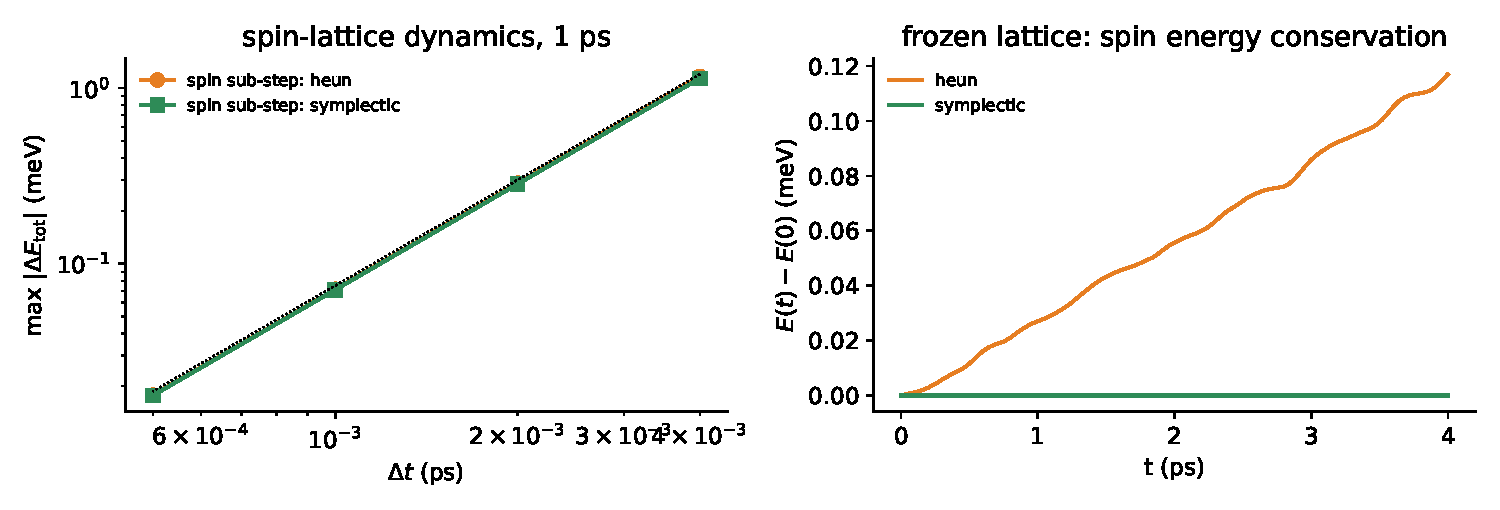
\includegraphics[width=0.92\textwidth]{figs/eng_sld.pdf}
\takeaway{with the palindromic splitting the total energy error falls as $\Delta t^2$; the symplectic spin step conserves the spin energy four orders of magnitude better than Heun.}
\end{frame}

\begin{frame}{Anharmonic lattice potentials \src{sld.py: SpinLattice(potential=...)}}
\begin{columns}[T]
\column{0.52\textwidth}
\small
Bond potentials $V(r)$, $x = r - r_0$, minimum at the reference bond length:
\[
\begin{aligned}
V_{\rm harm} &= \tfrac{\cJ k}{2}x^2\\
V_{\rm FPU} &= \tfrac{\cJ k}{2}x^2 + \tfrac{\cJ{k_3}}{3}x^3 + \tfrac{\cJ{k_4}}{4}x^4\\
V_{\rm Morse} &= \cJ D\big(1-e^{-\cJ a x}\big)^2\\
V_{\rm LJ} &= 4\cJ\varepsilon\Big[\big(\tfrac{\sigma}{r}\big)^{12}-\big(\tfrac{\sigma}{r}\big)^{6}\Big]+\cJ\varepsilon,\ \ \sigma = r_0/2^{1/6}
\end{aligned}
\]
forces $\bm F_i = \sum_j\big[V'(r_{ij}) - 2\cJ J'(r_{ij})\e_i\!\cdot\!\e_j\big]\hat{\bm r}_{ij}$.
\column{0.46\textwidth}
\begin{plainbox}{cK}
\small The cubic term ($k_3<0$, Morse) makes the bonds expand on heating: thermal expansion and its coupling
to the exchange, $J(r)$, enter the spin dynamics directly (magnetovolume effects, phonon--magnon damping).
\end{plainbox}
\begin{plainbox}{cJ}
\small\textbf{Checks}: forces = $-\partial\mathcal H/\partial\bm u$ to $10^{-8}$; with the palindromic splitting the energy error falls by $4.0\times$ per halving of $\Delta t$ for every potential.
\end{plainbox}
\end{columns}
\end{frame}

% ---------------------------------------------------------------------
\section{Part IV -- Statistical mechanics}
% ---------------------------------------------------------------------

\begin{frame}{Monte Carlo moves \src{montecarlo.py, fast.py}}
\begin{columns}[T]
\column{0.5\textwidth}
\small
\textbf{Graph colouring}: sites of one colour share no coupling, so a colour is updated in parallel and exactly.
Local change for $\e_i\to\e_i'$:
\[
\Delta\cE E = -\cH{\bm H}_i\!\cdot\!(\e_i'-\e_i) + \Delta\cE E_i^{\rm on\text{-}site},\ \ \cH{\bm H}_i = 2\sum_j\J_{ij}\e_j + \mu_B\mu_i\cH{\bm B}
\]
accepted with $\min(1,e^{-\beta_i\Delta\cE E})$.\\[4pt]
Moves: adaptive Gaussian cone (acceptance $\to50\%$), uniform, Hinzke--Nowak mixture, heat bath; over-relaxation $\e' = 2\frac{\e\cdot\cH{\bm H}}{|\cH{\bm H}|^2}\cH{\bm H}-\e$ (conserves $\cH{\bm H}\!\cdot\!\e$).
\column{0.48\textwidth}
\begin{eqbox}[Heat bath for the linear field]{cE}
\small
Sample $p(\e)\propto e^{\beta\cH{\bm H}\cdot\e}$ exactly: with $x=\beta|\cH{\bm H}|$, $u\in(0,1)$,
\[
\cos\cR\theta = 1 + \frac{1}{x}\ln\!\big[1-u\,(1-e^{-2x})\big],\quad\cR\phi = 2\pi u'
\]
then accept with $e^{-\beta\,\Delta\cE E^{\rm on\text{-}site}}$ (independence sampler $\Rightarrow$ detailed balance).
Acceptance $\approx 1$ for weak anisotropy.
\end{eqbox}
\end{columns}
\end{frame}

\begin{frame}{Exact Monte Carlo with long-range dipoles}
\begin{columns}[T]
\column{0.53\textwidth}
\small
Simultaneous updates of a colour are not exact when all spins interact. magex keeps the dipolar field and updates it after every accepted single-spin move ($\mathcal O(N)$):
\[
\cH{\bm B}^{\rm dip}_k \;\mathrel{+}=\; \cK W_{s_ks_j}(\bm c_k-\bm c_j)\,\mu_j\,\Delta\e_j\quad\forall k
\]
Energy change including the coupling of $j$ to its own periodic images $\cK W^0_j$:
\[
\Delta\cE E^{\rm dip} = -\mu_B\mu_j\,\Delta\e_j\!\cdot\!\big(\cH{\bm B}_j - \mu_j\cK W^0_j\e_j\big) - \frac{\mu_B\mu_j^2}{2}\Delta\big(\e_j\!\cdot\!\cK W^0_j\e_j\big)
\]
The field is rebuilt by FFT every sweep (no drift).
\column{0.45\textwidth}
\begin{plainbox}{cJ}
\small\textbf{Test}: periodic film with strong dipoles; brute-force Metropolis on full energies vs the exact kernel: equal $\langle\cE E\rangle$ within $1\sigma$ (\texttt{tests/test\_fast.py}).
\end{plainbox}
\begin{plainbox}{cE}
\small\textbf{Parallel tempering}: swap $T_a\leftrightarrow T_b$ with $\min\big(1,e^{(\beta_a-\beta_b)(E_a-E_b)}\big)$.\\[2pt]
\textbf{Wang--Landau}: $\ln g(E)\mathrel{+}=\ln f$, flat histogram, $1/t$ schedule; $Z(T)=\sum_E g(E)e^{-\beta E}$.
\end{plainbox}
\end{columns}
\end{frame}

\begin{frame}{Constrained Monte Carlo and the anisotropy $K(T)$ \src{cmc.py}}
\begin{columns}[T]
\column{0.53\textwidth}
\small
Fix the direction $\hat{\bm n}$ of $\bm M = \sum\e_i$ (Asselin et al. 2010). Pair move: primary $i$ (Gaussian), compensating $j$ restores the transverse components; with $z\parallel\hat{\bm n}$,
\[
e'_{j,xy} = e_{j,xy} + e_{i,xy} - e'_{i,xy},\quad e'_{jz} = \mathrm{sgn}(e_{jz})\sqrt{1-e_{jx}'^2-e_{jy}'^2}
\]
\[
P = \min\Big[1,\ \Big(\frac{M_z'}{M_z}\Big)^2\frac{|e_{jz}|}{|e'_{jz}|}\,e^{-\beta\Delta\cE E}\Big]
\]
The internal torque gives the free energy: $\langle\bm\tau\rangle\cdot\hat{\bm\theta} = -\partial\cE F/\partial\cR\theta$; uniaxial: $\langle\tau\rangle = -K(T)\sin2\cR\theta$.
\column{0.45\textwidth}
\small
Supported: exchange tensors, DMI, single-ion and surface anisotropy, cubic and higher uniaxial terms, Zeeman, and exact dipoles (incremental field).\\[4pt]
\begin{plainbox}{cK}
\small Callen--Callen: single-ion $K(T)/K(0)\simeq m^{l(l+1)/2} = m^3$ for $l=2$.
Film with dipoles only: torque at $\cR\theta=45^\circ$ equals $E_\perp-E_\parallel$ (shape anisotropy) to $<1\%$.
\end{plainbox}
\end{columns}
\end{frame}

\begin{frame}{Monte Carlo checks}
\centering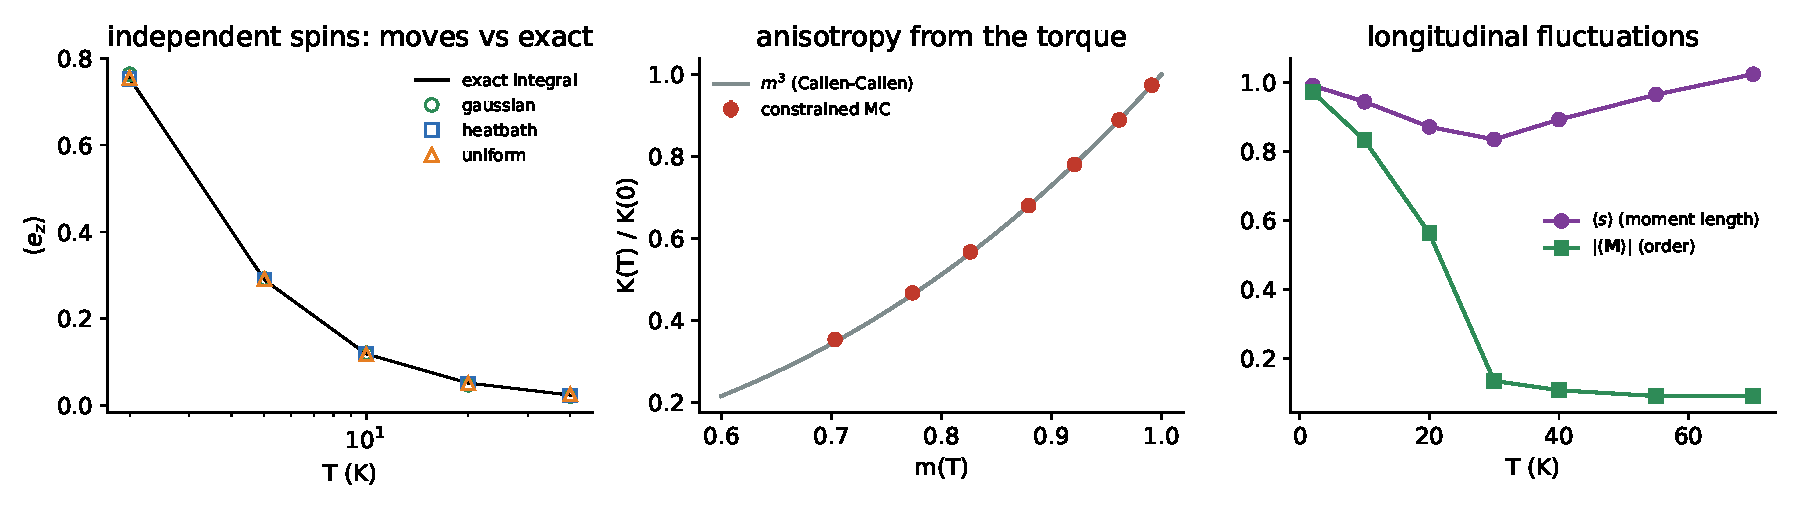
\includegraphics[width=\textwidth]{figs/eng_mc.pdf}
\takeaway{all move types reproduce exact single-spin averages; constrained MC follows $m^3$; longitudinal fluctuations keep a finite moment above $T_C$ while the order vanishes.}
\end{frame}

\begin{frame}{Ordering temperatures: finite-size scaling}
\begin{columns}[T]
\column{0.5\textwidth}
\small
Per spin: $\cE E$, $C = \frac{\langle E^2\rangle-\langle E\rangle^2}{Nk_BT^2}$, order parameter $m = |\sum_is_i\e_i|/N$ (signs from the magex reference: FM, AFM, ferrimagnet),
\[
\chi = \frac{N(\langle m^2\rangle-\langle m\rangle^2)}{k_BT},\qquad U_4 = 1-\frac{\langle m^4\rangle}{3\langle m^2\rangle^2}
\]
$T_C$ from Binder-cumulant crossings of two sizes; error bars by blocking.
\column{0.48\textwidth}
\begin{plainbox}{cE}
\small simple-cubic Heisenberg, $J=1$ meV (magex): exact $T_C = 1.443\cdot 2J/k_B = 33.49$ K; magex 33.29 K.\\[3pt]
bcc Fe (MFT exchange, $r_c=11$ \AA): 1060 K (exp. 1043 K).\\[3pt]
The J($\bm q$) stability check warns when a truncated coupling set makes a spiral the ground state.
\end{plainbox}
\end{columns}
\end{frame}

% ---------------------------------------------------------------------
\section{Part V -- Energy landscapes}
% ---------------------------------------------------------------------

\begin{frame}{Minimisation on $(S^2)^N$ \src{minimize.py}}
\begin{columns}[T]
\column{0.5\textwidth}
\small
Tangent gradient $\bm g_i = (\mathbb 1-\e_i\e_i^T)\,\partial\cE E/\partial\e_i$; convergence: $\max_i|\bm g_i|<\epsilon$.
Geodesic retraction for a tangent step $\bm d_i$:
\[
\e_i\to\e_i\cos|\bm d_i| + \hat{\bm d}_i\sin|\bm d_i|
\]
\textbf{L-BFGS} (Spirit's LBFGS-OSO idea): two-loop recursion on tangent vectors, pairs $(\bm s,\bm y)$ transported by projection, Armijo line search with max angle $0.3$ rad.\\
\textbf{NCG}: Polak--Ribière$^+$ $\beta = \max\big(0,\frac{\bm g'\cdot(\bm g'-\bm g)}{\bm g\cdot\bm g}\big)$, restarts.\\
\textbf{VP}: quick-min velocity projection.
\column{0.48\textwidth}
\begin{plainbox}{cK}
\small When $|\Delta\cE E|<10^{-11}|\cE E|$ (round-off), steps are accepted if the tangent gradient decreases: torques of $10^{-7}$ meV are reached for $10^4$ spins.
\end{plainbox}
\begin{eqbox}[GNEB with climbing image]{cR}
\small
$\bm F_\nu = -\nabla\cE E|_\perp + k\,(|\Delta_+|-|\Delta_-|)\,\hat{\bm\tau}_\nu$,\\
climbing image: $-\nabla\cE E + 2(\nabla\cE E\!\cdot\!\hat{\bm\tau})\hat{\bm\tau}$;
geodesic distances, upwind tangents, projected velocity Verlet.
\end{eqbox}
\end{columns}
\end{frame}

\begin{frame}{Harmonic analysis: Hessian and magnon eigenmodes \src{htst.py}}
\begin{columns}[T]
\column{0.53\textwidth}
\small
Tangent frame $(\bm t_{i1},\bm t_{i2})\perp\e_i$; Riemannian Hessian
\[
\cK H_{(ia),(jb)} = \bm t_{ia}\!\cdot\!\frac{\partial^2\cE E}{\partial\e_i\partial\e_j}\!\cdot\!\bm t_{jb} - \delta_{ij}\delta_{ab}\,\e_i\!\cdot\!\frac{\partial\cE E}{\partial\e_i}
\]
\textbf{Sparse}: $-2\J + 2\A$ + on-site terms analytic, dipolar and higher order matrix-free (gradient differences).\\[4pt]
Undamped linearised LLG: $\dot{\bm q} = \cK G\cK H\bm q$, $\cK G = \Gamma J$, $\Gamma_i = \gamma/(\mu_i\mu_B)$, $J=\begin{psmallmatrix}0&1\\-1&0\end{psmallmatrix}$ per spin.
\column{0.45\textwidth}
\begin{eqbox}[Frequencies as a symmetric problem]{cM}
\small
$\cK G\cK H$ has eigenvalues $\pm i\cM\omega$. With $\bm y = \cK H\bm q$:
\[
(\cK G^T\cK H\cK G)\,\bm y = \cM\omega^2\,\cK H^{-1}\bm y
\]
symmetric, $\cK H^{-1}$ positive definite at a minimum $\Rightarrow$ shift-invert Lanczos with sparse LU of $\cK H$.
\end{eqbox}
\footnotesize 22\,500-spin film: lowest modes in 10 s; $k=0$ mode equals $\gamma B/2\pi$; FM ring: analytic magnon dispersion to $10^{-8}$.
\end{columns}
\end{frame}

\begin{frame}{Harmonic transition-state theory with zero modes}
\begin{eqbox}[HTST rate (Bessarab, Uzdin \& Jónsson 2012)]{cE}
\[
k = \frac{v}{2\pi}\sqrt{\frac{\prod'\varepsilon^{\rm min}_i}{\prod''\varepsilon^{\rm sp}_i}}\,(2\pi k_BT)^{\frac{n_0^{\rm min}-n_0^{\rm sp}}{2}}\,\frac{V^{\rm sp}}{V^{\rm min}}\,e^{-\Delta\cE E/k_BT},
\qquad v^2 = \sum_{i\ \rm stable}\frac{a_i^2}{\varepsilon_i^{\rm sp}},\ \ a_i = \varepsilon^{\rm sp}_i\,\bm q_1\!\cdot\!\frac{\cK G}{1+\alpha^2}\bm q_i
\]
\end{eqbox}
\begin{columns}[T]
\column{0.5\textwidth}
\small
$\prod'$, $\prod''$ skip zero modes (and the unstable mode $\bm q_1$). Translational zero modes: generators $\partial\e/\partial x_a$ from the lattice gradients,
\[
V = \Big(\prod_a L_a\Big)\sqrt{\det\big(\partial_a\e\cdot\partial_b\e\big)}
\]
\column{0.48\textwidth}
\small
\textbf{Checks}: biaxial macrospin: prefactor = $f_{\rm FMR}$ of the minimum (exact); adding a decoupled free spin with zero modes at both points leaves $k$ unchanged.\\[3pt]
\textbf{Saddle polishing}: L-BFGS for the minimum; minimum-mode following (small systems) or Newton steps on the sparse Hessian (large systems) from the climbing image.
\end{columns}
\end{frame}

\begin{frame}{HTST without dense diagonalisation \src{htst.py: htst\_rate\_sparse}}
\begin{columns}[T]
\column{0.55\textwidth}
\small
\textbf{Determinants.} With the $k$ lowest modes $\lambda_i$ from shift-invert Lanczos and a tiny shift $s$:
\[
\ln|{\det}'\cK H| = \ln|\det(\cK H+s)| - \!\!\sum_{i\le k,\ \rm drop}\!\!\ln|\lambda_i+s| - \!\!\sum_{i\le k,\ \rm keep}\!\!\ln\Big|1+\frac{s}{\lambda_i}\Big|
\]
$\ln|\det(\cK H + s)|$ from the diagonal of a fill-reducing sparse LU; neglected remainder $< N s/\lambda_{\rm min}$.\\[4pt]
\textbf{Dynamical factor} from the unstable mode alone:
\[
v^2 = \sum_i\varepsilon_i(\bm q_1\!\cdot\!\cK G\bm q_i)^2 = (P\bm w)^T\cK H_{\rm sp}(P\bm w),\quad \bm w = \cK G^T\bm q_1
\]
($P$ removes $\bm q_1$ and the zero modes).
\column{0.43\textwidth}
\small
\textbf{Saddle multiplicity.} A free skyrmion has two translational zero modes, the collapsed saddle is pinned by the lattice: each lattice translation is a separate channel, $k\to N_{\rm cells}\,k$.
\vspace{3pt}

\centering\footnotesize
\begin{tabular}{rll}
\toprule
spins & prefactor (Hz) & time \\
\midrule
400 & $3.87\times10^{13}$ & 0.1 s \\
3\,600 & $3.763\times10^{13}$ & 0.6 s \\
14\,400 & $3.763\times10^{13}$ & 5.5 s \\
40\,000 & $3.763\times10^{13}$ & 37 s \\
\bottomrule
\end{tabular}

\raggedright sparse = dense to $10^{-8}$; box-size independent.
\end{columns}
\end{frame}

\begin{frame}{Skyrmion collapse: path and harmonic spectra}
\centering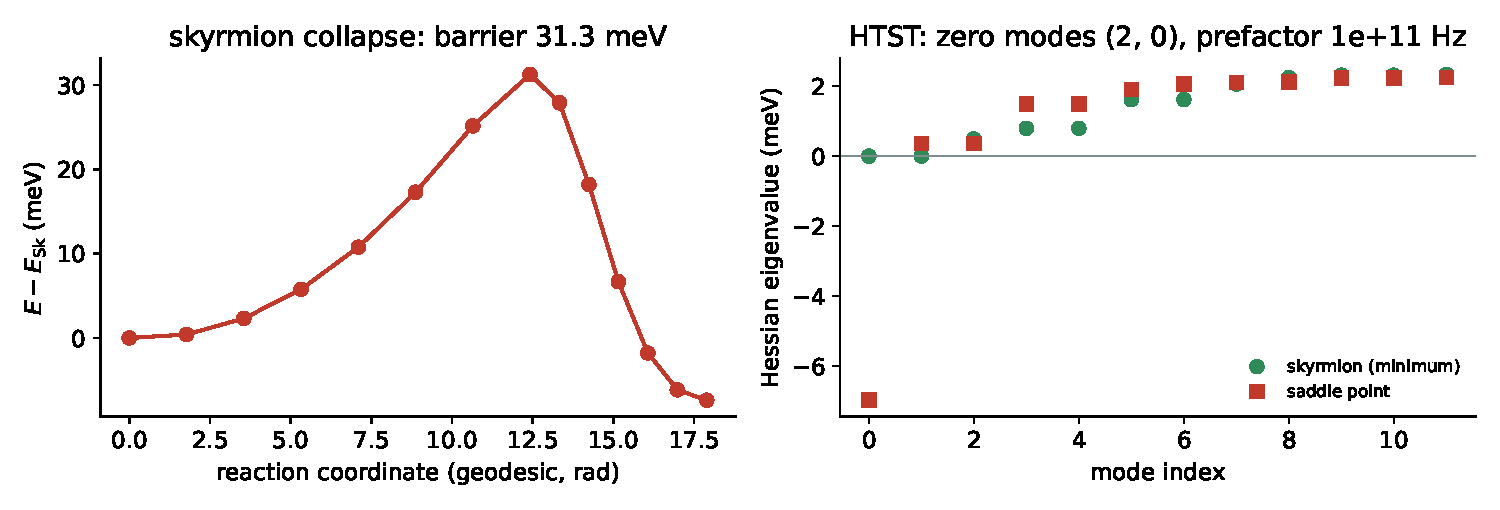
\includegraphics[width=0.92\textwidth]{figs/eng_landscape.pdf}
\takeaway{the isolated skyrmion has two translational zero modes; at the collapsed saddle they are lifted by the lattice (Peierls pinning), which HTST accounts for automatically.}
\end{frame}

% ---------------------------------------------------------------------
\section{Part VI -- Micromagnetics}
% ---------------------------------------------------------------------

\begin{frame}{Micromagnetic energy functional \src{micromag/system.py}}
\begin{eqbox}[Energy density (J/m$^3$)]{cJ}
\small
\[
\begin{aligned}
w ={}& A|\nabla\bm m|^2 + D_{\rm int}\big[m_z\nabla\!\cdot\!\bm m-(\bm m\!\cdot\!\nabla)m_z\big] + D_{\rm bulk}\,\bm m\!\cdot\!(\nabla\times\bm m)
 - K_{u1}(\bm m\!\cdot\!\bm u)^2 - K_{u2}(\bm m\!\cdot\!\bm u)^4\\
&+ K_{c1}\sum_{a<b}\alpha_a^2\alpha_b^2 + K_{c2}\,\alpha_1^2\alpha_2^2\alpha_3^2 + K_{c3}\Big(\sum_{a<b}\alpha_a^2\alpha_b^2\Big)^2
 + B_1\sum_a\epsilon_{aa}m_a^2 + 2B_2\sum_{a<b}\epsilon_{ab}m_am_b\\
&- M_s\bm m\!\cdot\!\cH{\bm B} - \frac{\mu_0}{2}M_s\bm m\!\cdot\!\bm H_d + w_{\rm custom}(\bm m,\bm r,t)
\end{aligned}
\]
\end{eqbox}
\begin{columns}[T]
\column{0.5\textwidth}
\small
$\cH{\bm B}_{\rm eff} = -\frac{1}{M_s}\frac{\delta w}{\delta\bm m}$; e.g.\ magnetoelastic
$B_x = -\frac{2}{M_s}\big[B_1\epsilon_{xx}m_x + B_2(\epsilon_{xy}m_y+\epsilon_{xz}m_z)\big]$.
Energies from fields: $E_k = -c_k\int M_s\bm m\cdot\cH{\bm B}_k$, $c = \tfrac12$ (quadratic), $\tfrac14$, $\tfrac16$, $\tfrac18$ (quartic, sextic, octic cubic terms).
\column{0.48\textwidth}
\small
Custom terms: $w_{\rm custom}$ given as a numpy expression; its field by central differences in $\bm m$.
All terms are tested against finite differences of the discrete energy.
\end{columns}
\end{frame}

\begin{frame}{Discretisation: exchange, DMI and boundaries}
\begin{columns}[T]
\column{0.47\textwidth}
\small
Exchange with link constants (harmonic mean, inter-region scaling):
\[
\cH{\bm B}^{\rm ex}_i = \frac{2}{M_{s,i}}\sum_{a,\pm}s_a\frac{A^\pm_{i,a}}{d_a^2}(\bm m_{i\pm a}-\bm m_i)
\]
Free surfaces: ghost cells from the chiral boundary condition
\[
2A\,\partial_{\bm n}\bm m = D_{\rm int}\big[(\bm m\!\cdot\!\bm n)\hat z - m_z\bm n\big] + D_{\rm bulk}\,\bm n\times\bm m
\]
\column{0.44\textwidth}
\begin{eqbox}[Energy-consistent DMI for varying $D$]{cJ}
\small
Cell-centred $D_i(\bm m_{i+1}-\bm m_{i-1})/2d$ is not the gradient of any discrete energy when $D$ varies.
Link form:
\[
D\,\partial_x\bm m\to\frac{D^+_i\bm m_{i+1}-D^-_i\bm m_{i-1}}{2d}
\]
with $D^\pm_i = \tfrac12(D_i+D_{i\pm1})$, or the \texttt{inter\_dmi} value across region boundaries. Field = exact energy derivative (error $10^{-10}$, was 50\%).
\end{eqbox}
\end{columns}
\end{frame}

\begin{frame}{Demagnetising field and solvers \src{demag.py, solver.py}}
\begin{columns}[T]
\column{0.5\textwidth}
\small
\[
\bm H_d(\bm r_i) = -\sum_j\cK N(\bm r_i-\bm r_j)\,M_s\bm m_j
\]
Newell cell-averaged tensor (asymptotic far field), six components, FFT convolution with zero padding; periodic axes by macro-geometry image sums.
The tensor is symmetric: 6 independent components in Fourier space.\\[3pt]
\texttt{precision = "single"}: FFTs in float32 as on mumax3 GPUs, $2\times$ faster, $|\Delta H_d|/|H_d|\sim2\times10^{-7}$.\\[3pt]
Edge smoothing: sub-cell volume fractions $\phi_i$ in $M_s\phi_i\bm m_i$ for the demag field.
\column{0.48\textwidth}
\begin{eqbox}[Solvers]{cR}
\small
adaptive Dormand--Prince RK45 (FSAL) and Bogacki--Shampine RK23:
$\Delta t' = 0.9\,\Delta t\,(\mathrm{tol}/\mathrm{err})^{1/p}$;
fixed-step Heun (thermal), RK4, RK2, Euler; Barzilai--Borwein minimiser; relax; hysteresis.
\end{eqbox}
\small Moving frame (mumax3 \texttt{ext\_centerWall}): wall offset $x_w - L/2 = \mathrm{sgn}(m_c^{\rm left})\langle m_c\rangle L/2$, shift by whole cells, record lab-frame position.
\end{columns}
\end{frame}

\begin{frame}{Spin torques in the continuum \src{micromag/stt.py, fp\_torques.py}}
\begin{columns}[T]
\column{0.5\textwidth}
\begin{eqbox}[Spin--orbit torque]{cS}
\small
\[
\cH{\bm B}_{\rm SOT} = B_{\rm DL}\,\bm m\times\bm\sigma + B_{\rm FL}\,\bm\sigma,\qquad B_{\rm DL} = \frac{\hbar\,\theta_{\rm eff}J}{2eM_st}
\]
damping-like torque $-\gamma B_{\rm DL}\,\bm m\times(\bm m\times\bm\sigma)$ pushes $\bm m$ towards $\bm\sigma$.
From first principles: $\theta_{\rm eff} = 2\sigma_{\rm SH}/\sigma_{xx}$ (orbital Hall via $\eta_{LS}$).
\end{eqbox}
\begin{eqbox}[Spin pumping]{cS}
\small
\[
\Delta\alpha = \frac{g\mu_B\,g_r^{\uparrow\downarrow}}{4\pi M_s t},\qquad
\bm j_s = \frac{\hbar}{4\pi}g_r^{\uparrow\downarrow}\,\bm m\times\dot{\bm m}
\]
\end{eqbox}
\column{0.48\textwidth}
\begin{eqbox}[Zhang--Li and Slonczewski]{cS}
\small
\[
\bm u = \frac{Pg\mu_B\bm J}{2eM_s(1+\beta^2)}
\]
\[
\epsilon(\bm m) = \frac{P\Lambda^2}{(\Lambda^2+1)+(\Lambda^2-1)\,\bm m\!\cdot\!\bm p}
\]
\end{eqbox}
\begin{eqbox}[Thiele equation]{cK}
\small
\[
\bm G\times(\bm v-\bm u) + \cK{\mathcal D}\,(\alpha\bm v-\beta\bm u) = 0
\]
$\bm G = 4\pi Q\,\hat z$, $\cK{\mathcal D}_{ij} = \int\partial_i\bm m\cdot\partial_j\bm m\,dA$; predicted velocity and skyrmion Hall angle.
\end{eqbox}
\end{columns}
\end{frame}

\begin{frame}{Two-sublattice micromagnetics: antiferromagnets and altermagnets \src{micromag/afm.py}}
\begin{columns}[T]
\column{0.55\textwidth}
\begin{eqbox}[Energy density]{cJ}
\small
\[
w = \sum_{s=A,B}w_s[\bm m_s] - \frac{J_{AF}}{t}\,\bm m_A\!\cdot\!\bm m_B + A_{AB}\,\nabla\bm m_A\!:\!\nabla\bm m_B
\]
each sublattice with its own $M_s$, $A$, $D$, $K$, $\alpha$; demag from $\bm M_A+\bm M_B$; one LLG per sublattice.
\end{eqbox}
\begin{eqbox}[d-wave altermagnet]{cJ}
\small
\[
A^{x}_{A} = A^{y}_{B} = A(1+\delta),\qquad A^{y}_{A} = A^{x}_{B} = A(1-\delta)
\]
splits the two magnon chiralities along $k_x$ and $k_y$ with opposite sign.
\end{eqbox}
\column{0.43\textwidth}
\small
\textbf{Checks}: uniform AFM resonance
\[
\omega_\pm = \gamma\Big[\sqrt{B_K(2B_E+B_K)}\pm B\Big]
\]
and the chirality-resolved spin-wave dispersion from the \texttt{dispersion} stage; AFM domain-wall velocity under SOT.
\end{columns}
\end{frame}

\begin{frame}{Finite temperature in the continuum: Landau--Lifshitz--Bloch \src{micromag/llb.py}}
\begin{columns}[T]
\column{0.55\textwidth}
\begin{eqbox}[LLB equation (Garanin)]{cE}
\small
\[
\dot{\bm m} = -\gamma\bm m\times\cH{\bm B} + \frac{\gamma\alpha_\parallel}{m^2}(\bm m\!\cdot\!\cH{\bm B})\,\bm m - \frac{\gamma\alpha_\perp}{m^2}\,\bm m\times(\bm m\times\cH{\bm B})
\]
\[
\alpha_\parallel = \lambda\frac{2T}{3T_C},\quad \alpha_\perp = \lambda\Big(1-\frac{T}{3T_C}\Big)\ (T<T_C)
\]
\[
\cH{\bm B}_\parallel = \frac{1}{2\chi_\parallel}\Big(1-\frac{m^2}{m_e^2}\Big)\bm m\quad (T<T_C)
\]
\end{eqbox}
\column{0.43\textwidth}
\small
Mean field: $m_e = L(3T_Cm_e/T)$, $\chi_\parallel = \frac{\mu_s}{k_BT}\frac{L'(x)}{1-\frac{3T_C}{T}L'(x)}$.\\[4pt]
\textbf{Callen--Callen scaling} of the $T=0$ parameters:
\[
M_s\propto m_e,\ A,D\propto m_e^{1.8},\ K\propto m_e^{3}
\]
with $m_e(T)$ from mean field or from a magex Monte Carlo run. Two-temperature model for ultrafast demagnetisation.
\end{columns}
\end{frame}

\begin{frame}{Micromagnetics: moving frame and kernel speed}
\centering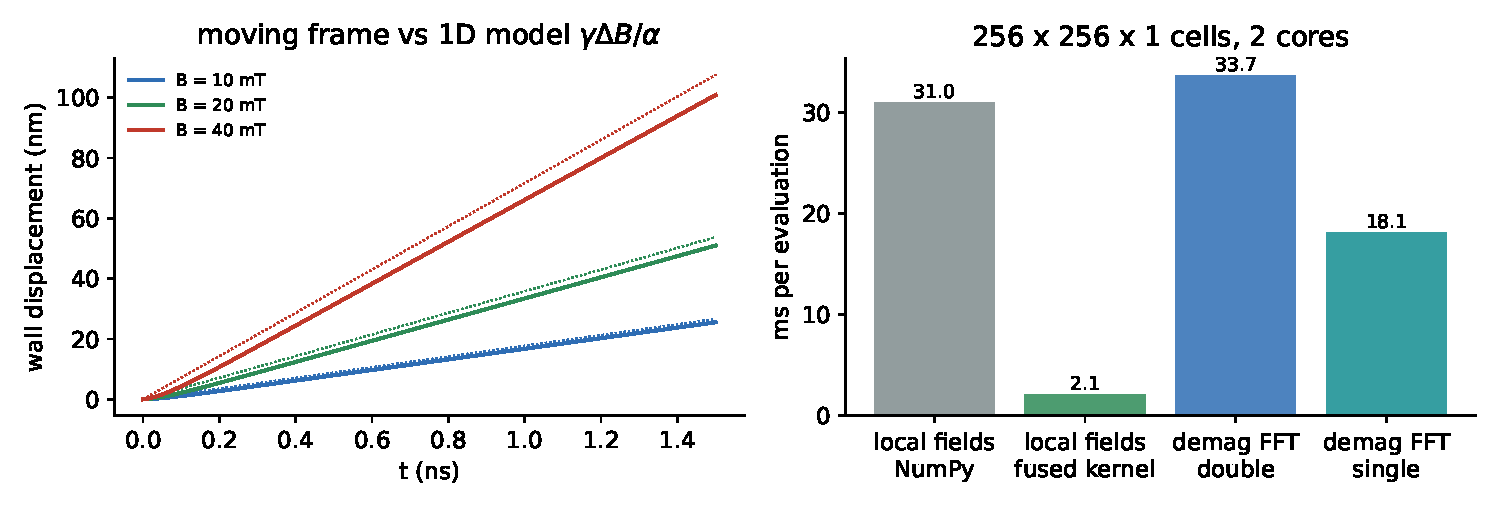
\includegraphics[width=0.92\textwidth]{figs/eng_micromag.pdf}
\takeaway{the moving frame follows the 1D-model wall velocity; the fused local-field kernel is 15$\times$ faster than the NumPy stencil, so the demag FFT dominates.}
\end{frame}

% ---------------------------------------------------------------------
\section{Part VII -- Implementation, performance, validation}
% ---------------------------------------------------------------------

\begin{frame}{Multithreaded kernels \src{fast.py}}
\begin{columns}[T]
\column{0.52\textwidth}
\small
\textbf{Symmetry-reduced couplings.} The $3N\times3N$ CSR matrix becomes a neighbour list; every distinct 3$\times$3 block is stored once (translational invariance) and classified:
\[
\J_{ij}\in\begin{cases}J\mathbb 1 & 1\ \text{number}\\ J\mathbb 1 + [\Dv]_\times & 4\ \text{numbers}\\ \text{general} & 9\ \text{numbers}\end{cases}
\]
8 bytes of memory traffic per neighbour.\\[4pt]
\textbf{Fused steps.} Heun = two passes: (noise + field + predictor), (field at predictor + corrector + norm).
Monte Carlo colours swept in parallel; serial twins below 2048 sites.
\column{0.46\textwidth}
\begin{eqbox}[Reproducible parallel random numbers]{cE}
\small
xorshift64$^*$ streams on 256 fixed chunks of the site list (results independent of the number of threads);
normals by the Marsaglia--Tsang ziggurat (128 layers): one 32-bit draw and one comparison in 98.8\% of calls.
\end{eqbox}
\small All kernels agree with the NumPy reference to $10^{-15}$; MC checked against exact single-spin integrals.
\end{columns}
\end{frame}

\begin{frame}{Speed and agreement with VAMPIRE, UppASD and Spirit}
\centering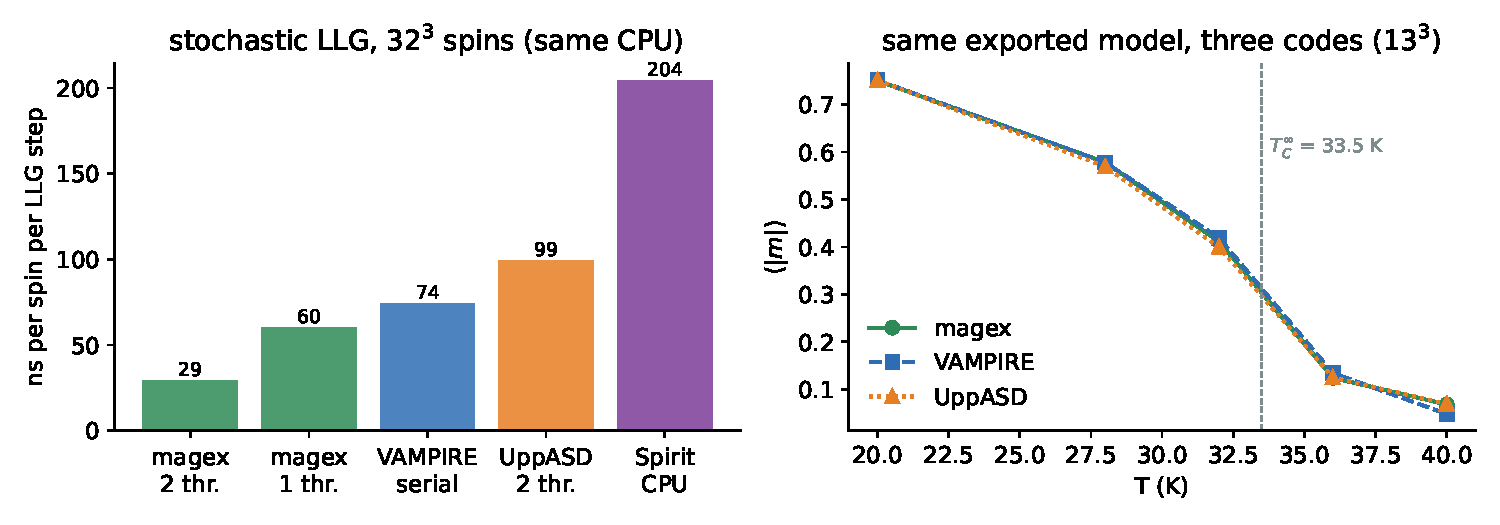
\includegraphics[width=0.93\textwidth]{figs/eng_bench.pdf}
\vspace{-4pt}
\begin{columns}[T]
\column{0.5\textwidth}
\footnotesize All codes built from source on the same 2-core CPU; VAMPIRE serial, UppASD OpenMP, Spirit CPU.
MC: magex 80 (1 thread) / 50 (2 threads) ns per spin-sweep vs VAMPIRE 110.
\column{0.48\textwidth}
\footnotesize Spirit: same energy for a perturbed skyrmion to $3\times10^{-8}$; UppASD: same LLG relaxation (0.917 vs 0.918).
Production GPU codes (VAMPIRE, Spirit CUDA, mumax3) remain ahead until magex's CUDA kernels are timed on hardware.
\end{columns}
\end{frame}

\begin{frame}{Distributed memory: MPI domain decomposition \src{mpi\_spin.py}}
\begin{columns}[T]
\column{0.53\textwidth}
\small
Slabs along the longest supercell axis. Rank $r$ owns sites $\mathcal O_r$ and keeps ghosts
$\mathcal G_r = \{j\notin\mathcal O_r : \J_{ij}\neq0,\ i\in\mathcal O_r\}$; local matrix = owned rows only.
\[
\underbrace{\text{noise + field + predictor}}_{\text{own sites}} \to \text{halo}(\tilde\e) \to \underbrace{\text{corrector}}_{\text{own}} \to \text{halo}(\e)
\]
Monte Carlo: every global colour group is split among the ranks, one halo exchange per colour, so the
algorithm is exactly the serial one. Non-blocking point-to-point messages; energies and moments by
\texttt{allreduce}.
\column{0.45\textwidth}
\centering\footnotesize
\begin{tabular}{lcc}
\toprule
131\,072 spins & LLG & MC \\
 & ns/spin/step & ns/spin/sweep\\
\midrule
1 rank & 53.8 & 71.9 \\
2 ranks & 30.4 & 39.1 \\
speed-up & 1.77 & 1.84 \\
\bottomrule
\end{tabular}

\vspace{6pt}
\begin{plainbox}{cJ}
\raggedright\small $T=0$ trajectory with 2 ranks = serial to $2\times10^{-15}$; set-up replicated on every rank.
\end{plainbox}
\end{columns}
\end{frame}

\begin{frame}{CUDA back end \src{cuda\_backend.py, micromag/gpu.py}}
\begin{columns}[T]
\column{0.52\textwidth}
\small
\textbf{Atomistic} (numba.cuda): one thread per spin; device twins of the CPU kernels:
\begin{itemize}\small
\item coupling table (1, 4 or 9 numbers per bond type), on-site tensors, cubic/higher uniaxial terms
\item fused Heun/Depondt predictor and corrector kernels; spins stay on the device
\item Metropolis / heat-bath colour sweeps, \texttt{atomicAdd} acceptance counter
\item per-thread xoroshiro128+ random streams
\end{itemize}
\textbf{Micromagnetics} (CuPy): all arrays on the device; the demag convolution runs through cuFFT, optionally in single precision.
\column{0.46\textwidth}
\begin{plainbox}{cK}
\small\textbf{Verification} in numba's CUDA simulator:
\begin{itemize}\small
\item $T=0$ LLG trajectories equal to the CPU kernels ($10^{-16}$)
\item Monte Carlo averages equal to the exact single-spin integral
\item thermal LLG runs agree with the CPU solver within statistics
\end{itemize}
\end{plainbox}
\begin{plainbox}{cJ}
\small No GPU was available: speed on hardware is still to be measured.
\end{plainbox}
\end{columns}
\end{frame}

\begin{frame}{Conventions when exchanging models with other codes \src{interop.py}}
\centering\small
\renewcommand{\arraystretch}{1.3}
\begin{tabular}{l l l}
\toprule
code & Hamiltonian & conversion from magex \\
\midrule
magex / TB2J & $-\sum_{i\neq j}[J\,\e\!\cdot\!\e + \Dv\!\cdot\!(\e\times\e) + \e\!\cdot\!\J^{S}\!\cdot\!\e]$ & meV / eV \\
UppASD & same, ordered pairs, mRy; $E_K = -K_1\sin^2\theta$ & $J/13.6057$; $K_1 = -K$ (easy axis) \\
VAMPIRE & tensorial UCF, joules, each bond once & $J_V = 2J\cdot1.602\times10^{-22}$ \\
Spirit & $-\sum_{\langle ij\rangle}[J\,\e\!\cdot\!\e+\Dv\!\cdot\!(\e\times\e)]$, unique pairs & $J_S = 2J$, $D_S = 2D$ ($\J^S$ dropped) \\
mumax3 & continuum (TOML $\to$ .mx3) & regions, CSG, $K_{c1-3}$, $B_{1,2}$, solvers \\
\bottomrule
\end{tabular}

\vspace{6pt}
\begin{plainbox}{cC}
\small Every keyword the exporters write was checked against the parsers in the VAMPIRE, UppASD and Spirit sources; structure, program and LLG settings are translated too (\texttt{create:sphere}, \texttt{dipole:solver = atomistic}, \texttt{do\_dip}, \texttt{ddi\_method fft}, \dots).
\end{plainbox}
\end{frame}

\begin{frame}{Validation summary}
\centering\scriptsize
\renewcommand{\arraystretch}{1.18}
\begin{tabular}{l l l}
\toprule
check & reference & magex \\
\midrule
FFT dipolar field (open, two sublattices) & direct pair sum & $10^{-16}$ \\
film shape anisotropy (thick film) & $\tfrac{\mu_0}{2}M_s^2V$ & $<1\%$ \\
exact dipolar MC & brute-force Metropolis & within $1\sigma$ \\
MC moves, independent spins & exact integral & within $1\sigma$ \\
constrained MC $K(T)$ & $m^3$ (Callen--Callen) & 0.5\% \\
LSD $\langle s\rangle$ & LSF Monte Carlo & $10^{-3}$ \\
integrators (Larmor) & analytic & $\mathcal O(\Delta t^2)$ \\
Zhang--Li wall velocity & $(\beta/\alpha)u$ & 2\% \\
FMR & Kittel & 0.1\% \\
HTST prefactor (biaxial spin) & $f_{\rm FMR}$ & $10^{-12}$ \\
sparse HTST (skyrmion) & dense HTST & $10^{-8}$ \\
MPI LLG, 2 ranks ($T=0$) & serial trajectory & $2\times10^{-15}$ \\
CUDA kernels (simulator) & CPU kernels & $10^{-16}$ \\
eigenfrequencies of a FM ring & analytic magnons & $10^{-8}$ \\
spin--lattice energy error & second order & ratio 4.0 per halving \\
micromag. terms (Kc2, Kc3, B$_1$, B$_2$, inter-DMI, custom) & finite differences & $10^{-9}$ \\
moving frame wall velocity & $\gamma\Delta B/\alpha$ & 3\% \\
m(T), simple cubic & VAMPIRE, UppASD & within critical fluctuations \\
energy of a skyrmion configuration & Spirit & $3\times10^{-8}$ \\
\bottomrule
\end{tabular}
\end{frame}

\begin{frame}[fragile]{Using the engine}
\begin{columns}[T]
\column{0.5\textwidth}
\scriptsize
\begin{verbatim}
[spinmodel]
results   = "magex_results/results.json"
supercell = [14, 14, 14]
pbc       = [false, false, false]

[structure]
shape      = "sphere"
size       = 20.0
core_shell = {radius = 12.0, core = "core",
              shell = "shell"}
materials  = [{name = "core", Kc = 0.02},
              {name = "shell", ks = 0.05}]
exchange_scale = [[1,1,1],[1,1,-0.3],[1,-0.3,0.6]]
dipolar    = true

[program]
type    = "field_cooling"
T_start = 60.0
field   = [0, 0, 1.0]
\end{verbatim}
\column{0.48\textwidth}
\scriptsize
\begin{verbatim}
magex run      input.toml   # exchange (Part I)
magex llg      llg.toml     # spin dynamics
magex mc       mc.toml      # T_C, PT, WL
magex program  prog.toml    # hysteresis, FMR,
                            # CMC, LSF, ...
magex gneb     gneb.toml    # barriers + HTST
magex sqw      sqw.toml     # S(q, w)
magex micromag mm.toml      # continuum
magex export   prog.toml --to vampire
               # | uppasd | spirit | mumax3
\end{verbatim}
\normalsize
\begin{plainbox}{cC}
\small Output: CSV, NPZ, VTK (ParaView), extended XYZ (OVITO), OVF 2.0, PDF/PNG figures.
\end{plainbox}
\end{columns}
\end{frame}
